\documentclass[tikz,border=10pt]{standalone}
\usepackage{tikz}
\begin{document}
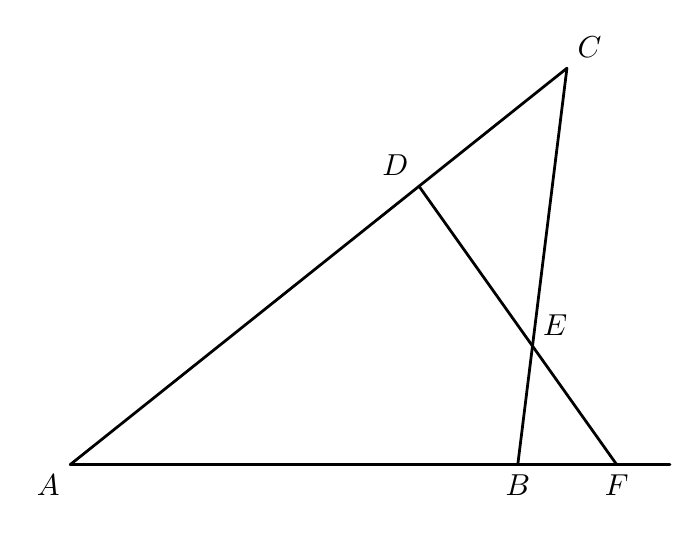
\begin{tikzpicture}[line width=1.0pt, line join=round, line cap=round]
  % Scale s = 0.008909 cm/px, origin at ink-bbox centre (527, 386.5) px
  % Named coordinates (converted from pixel positions)
  \coordinate (A) at (-3.608,-2.392);
  \coordinate (B) at (2.076,-2.392);
  \coordinate (F) at (3.332,-2.392);
  \coordinate (C) at (2.700,2.642);
  \coordinate (D) at (0.820,1.145);
  \coordinate (E) at (2.263,-0.886);
  \coordinate (Lend) at (4.009,-2.392);   % baseline right end (977 px)

  % Baseline: starts at A (5 px overhang trimmed), extends past F
  \draw (A) -- (Lend);
  % Segment A--C (passes through D)
  \draw (A) -- (C);
  % Segment C--B (passes through E)
  \draw (C) -- (B);
  % Segment D--F (passes through E)
  \draw (D) -- (F);

  % Labels (11 pt font, 13.2 pt leading)
  \node[below left, font=\fontsize{11}{13.2}\selectfont] at (A) {$A$};
  \node[below, font=\fontsize{11}{13.2}\selectfont] at (B) {$B$};
  \node[below, font=\fontsize{11}{13.2}\selectfont] at (F) {$F$};
  \node[above right, font=\fontsize{11}{13.2}\selectfont] at (C) {$C$};
  \node[above left, font=\fontsize{11}{13.2}\selectfont] at (D) {$D$};
  \node[above right, font=\fontsize{11}{13.2}\selectfont] at (E) {$E$};
\end{tikzpicture}
\end{document}